\newpage
\section{Denial of Service Attacks}

Suppose you operate a web site and would like to make your web site resilient to denial
of service (DoS) attacks (both conventional denial of service attacks, as well as
distributed DoS attacks).

Recall that many denial of service attacks are based on the principle of
asymmetry: without expending many resources, an attacker can cause the victim
to expend many more resources. In this question, we'll review various ways
asymmetry show up in DoS attacks, as well as various mechanisms you might use
to defend against them. Some of these techniques we have discussed in class.
Others may be new, but you should be able to reason through the attack and
defenses based on what we've taught you.

\prob{20} 
You notice that your
web server suddenly receives a flood of TCP SYN packets from many distinct IP
addresses. You realize that you forgot to enable TCP SYN cookies. 

\begin{enumerate}
\item Describe
what might happen to your server without TCP SYN cookies enabled. 
\item Describe why enabling TCP SYN cookies will help defend against the attack
you are witnessing.
\end{enumerate}
\eprob

\if 0
\newpage
\prob{20} After you enable TCP SYN cookies, you notice that your attacker has begun
launching a DDoS attack from many different IP addresses, whereby each IP address
is sending your web server a legitimate HTTP request. 
\begin{enumerate}
	\item Explain why this attack might be more difficult to detect and mitigate as
	compared to a SYN flood attack.
	\item Companies such as CloudFlare use mechanisms such as CAPTCHAs---images and
	words that are difficult for computers to decipher but easier for humans to read---to
	defend against these kinds of attacks. Briefly describe one advantage to using
	a CAPTCHA to defend against this type of DDoS attack; also describe {\em two} disadvantages
	to using CAPTCHAs (Hint: Think about who or what may not be able to solve CAPTCHAs.
	In case you don't know what a CAPTCHA is, it looks like the figure below.)

	\centering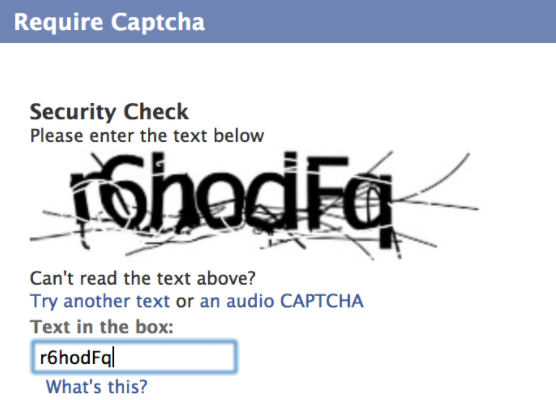
\includegraphics[width=0.3\linewidth]{captcha}
\end{enumerate}
\eprob
\fi

\newpage
\prob{20}
We discussed a large-scale DDoS attack
that was mounted from a collection of insecure Internet-connected DVR cameras on
October 21, 2016. The attack generated about 1.2 terabits per second of attack traffic
and managed to bring down
many web sites (including Twitter, Reddit, and others), {\em without directly sending
traffic to each of these web sites}. 
\begin{enumerate}
	\item Explain how the DDoS attack managed to bring down all of these web sites without
	sending attack traffic to each site directly.
	\item This particular attack did not use reflection or amplification. Suppose,
	however, that each Internet-connected device that participated in this attack had
	been running an open DNS resolver. Describe a modification to the attack that took
	place that could have resulted in an increase in the attack traffic by an order
	of magnitude.
%	\item How might the original attack (which was not a reflection attack) have been
%	prevented? In general, how might a reflection attack be prevented?
\end{enumerate}
\eprob